\begin{frame}{Dynamics}  %% ---------- Intro/motivation 
    \begin{tikzpicture}[overlay,remember picture]
        \uncover<1->{ % <-> |
            \node (t1) [anchor=center,scale=1,opacity=1] at ([shift={(-0.6cm,-0.0cm)}]current page.center){
                \parbox{1.\textwidth}{
                    Semi-analytic model (energy conservation) in a 
                    thin-shell  approximation:\\%\footcite{Nava:2013,Kumar:2014upa,Zhang:2018book}; \\
                    
                    %From stress-energy tensor %$ T^{\mu\nu} = (\rho' c^2 + p') u^{\mu}u^{\nu} + p' g^{\mu\nu}$ \\
                    %we write evolution equation: 
                    \vspace{-2mm}
                    \begin{equation*}
                        \begin{aligned}
                            dE_{\rm tot} = 0 \rightarrow & d [ \Gamma (M_0 + m) c^2 + \Gamma_{\rm eff}E_{\rm int}' ] = dm c^2 + \Gamma_{\rm eff} dE_{\rm rad}'. \\
                            & dE_{\rm int}' = dE_{\rm sh}' + dE_{\rm ad}' + dE_{\rm rad}',
                        \end{aligned}
                    \end{equation*}
                    
                    Adiabatic evolution, $\Gamma=f(R)$; \\
                    If $\rho_{\rm ISM}=\text{const}$: free-coasting ($\Gamma=\Gamma_0$), and deceleration,  $\Gamma\downarrow$.\\
                    
                    \textbf{Structure:} lateral, $\{\theta_i\}$, and velocity $\{\upsilon_i\}$; \\
                    \textbf{Initial conditions}: ejecta profile, \\
                    $\{ E_{ij, 0} \}=f(\Gamma_{i, 0},\theta_{j, 0})$. %($\Gamma=(1-\beta^2)^{-2}$); $\beta=\upsilon/c$; \\
                    %\textbf{Main stages:} free-coasting + deceleration; \\
                    %$\Gamma$ is the bulk Lorentz factor. \\
                    %\textbf{Shock properties}, $\rho_{\rm sh}$, $\beta_{\rm sh}$, $R_{\rm sh}$ \\
            }};
            
        }
        %        \uncover<1->{ % <-> |
            %            \node (t1) [anchor=center,scale=1,opacity=1] at ([shift={(4.0cm,-2.0cm)}]current page.center){
                %                \parbox{0.5\textwidth}{
                    %                    \textbf{Evolution}: free-coasting + deceleration; \\
                    %                    %Electrons accelerated to power-law distribution $\gamma_e^{-p}$
                    %                    Total energy in electrons and magnetic fields $\epsilon_e$, $\epsilon_B$;
                    %                    Assume for electrons local istropic distribution of angles relative $\vec{B}$; \\
                    %                    Assume $\vec{B}$ is random mix of orientations; \\
                    %                    Spectrum from a PL electrons is also PL; \\
                    %                    %Assume local cooling rate $=$ expansion time
                    %                    Emission is isotropic in the rest-frame
                    %                    %Intensity-weighted mean change in any charactersitic gets broadened
                    %            }};
            %        }
        % Margalit B., Quataert E., 2021, ApJL, 923, L14. 
        %        \uncover<1->{ % <-> |
            %            \node (t1) [anchor=center,scale=1,opacity=1] at ([shift={(-4.4cm,-2.4cm)}]current page.center){
                %                \parbox{0.5\textwidth}{
                    %                    \begin{equation*}
                        %                        P_{\nu'} = \int_{\gamma_{\nu'}}^{\infty} d\gamma_e \frac{dn'}{d\gamma_e}P_{s}'(\nu'); \hspace{3mm} \frac{dn'}{d\gamma_e} \propto
                        %                        \begin{cases}
                            %                            \gamma_e^{-2} &\text{s.c.} \\ 
                            %                            \gamma_e^{-p-1} &\text{f.c.}
                            %                        \end{cases}
                        %                    \end{equation*}
                    %                    %
                    %                    \begin{equation*}
                        %                        F(\nu,t) = \frac{1+z} {2d_L^2}\int_0^{\theta}\int_{0}^{r}\frac{P'(\nu',t_{\rm em},r)}{\Gamma^2(1-\beta\cos\theta)^2}r^2 dr d\cos\theta
                        %                    \end{equation*}
                    %                    \textbf{Synchrotron Radiation}
                    %            }};
            %        }
        
        %        \uncover<1-1>{ % <-> |
            %            \node (img1) [anchor=center,scale=1,opacity=1] at ([shift={(4.5cm,-0.3cm)}]current page.center){
                %                \parbox{0.6\textwidth}{
                    %                    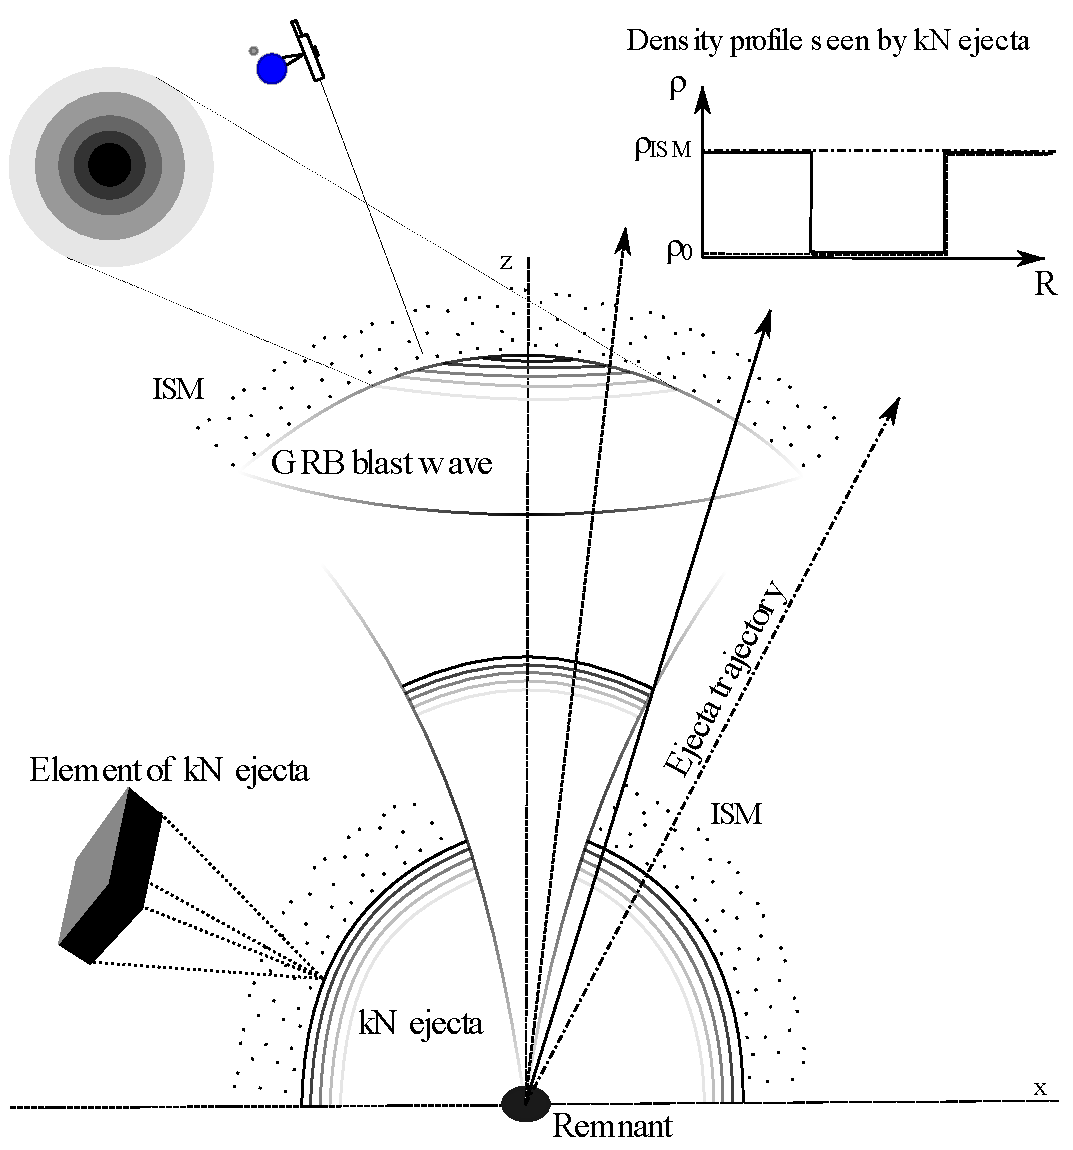
\includegraphics[height=7.8cm]{figures/structure2.pdf}
                    %                    %\includesvg[height=7.2cm]{figures/structure2}
                    %            }};
            %        }
        \uncover<1->{ % <-> |
            \node (img1) [anchor=center,scale=1,opacity=1] at ([shift={(5.0cm,-2.4cm)}]current page.center){
                \parbox{0.6\textwidth}{
                    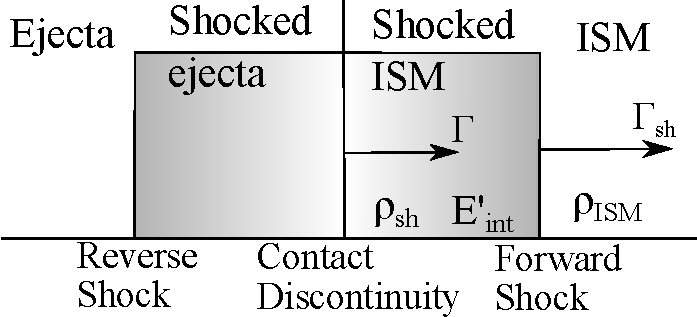
\includegraphics[height=3.0cm]{../figs/shock_scatch2.pdf}
            }};
            
        }
        
    \end{tikzpicture}
\end{frame}


\begin{frame}{Radiation}  %% ---------- Intro/motivation 
    \begin{tikzpicture}[overlay,remember picture]
        \uncover<1->{ % <-> |
            \node (t1) [anchor=center,scale=1,opacity=1] at ([shift={(-3.6cm,1.4cm)}]current page.center){
                \parbox{0.6\textwidth}{
                    \textbf{A shock}:\\%\footcite{Zhang:2018book}:%$^{\textcolor{gray}{\text{\cite{Rezzolla:2013,Kumar:2014upa,Zhang:2018book,Nava:2013}}}}$
                    \begin{itemize}
                        \item compresses fluid, $\rho_{\rm sh} = 4; \Gamma_{\rm sh} \rho_{\rm ISM}$;
                        \item amplifies magnetic fields, $B=\sqrt{8 \pi \epsilon_B e'}$;
                        \item accelerates electrons, $\frac{dn'}{d\gamma_e} \propto \gamma_e^{-p}$.
                    \end{itemize}
                    
            }};
            
        }
        \uncover<1->{ % <-> |
            \node (t1) [anchor=center,scale=1,opacity=1] at ([shift={(4.6cm,1.3cm)}]current page.center){
                \parbox{0.6\textwidth}{
                    \textbf{Synchrotron radiation spectrum} \\%$^{\textcolor{gray}{\text{\cite{Sari:1997qe}}}}$ \\
                    Broken power law (BPL)\\%\footcite{Sari:1997qe,Wijers:1998st}; \\ 
                    %$\nu_m\propto\gamma_m$, $\nu_c\propto\gamma_c$ \\
            }};
            
        }
        
        %        \uncover<1->{ % <-> |
            %            \node (t1) [anchor=center,scale=1,opacity=1] at ([shift={(-4.4cm,-1.7cm)}]current page.center){
                %                \parbox{0.5\textwidth}{
                    %                    \textbf{Electron spectrum}: %$^{\textcolor{gray}{\text{\cite{Sari:1997qe}}}}$ \\
                    %                    broken power law (BPL) with 
                    %                    \vspace{-3mm}
                    %                    \begin{equation*}\label{eq:method:gm_pl_only}
                        %                        \gamma_m' = \frac{p-2}{p-1} \frac{\epsilon_e e'}{n' m_e c^2} \hspace{3mm} 
                        %                        \gamma_c' = \frac{6 \pi m_e c \Gamma}{\sigma_T t_{\rm em} B'^2}, \hspace{3mm}
                        %                        %e' = \frac{E_{\rm int}'}{V'}
                        %                    \end{equation*}
                    %                \vspace{-5mm}
                    %                    \begin{footnotesize}
                        %                        \begin{itemize}
                            %                            \item Slow cooling $\gamma_m' < \gamma_c'$
                            %                            \item Fast cooling $\gamma_m' > \gamma_c'$
                            %                        \end{itemize}
                        %                    \end{footnotesize}
                    %            }};
            %        }
        \uncover<1->{ % <-> |
            \node (t1) [anchor=center,scale=1,opacity=1] at ([shift={(-4.4cm,-1.5cm)}]current page.center){
                \parbox{0.5\textwidth}{
                    \textbf{Spectral breaks}: 
                    \begin{itemize}
                        \item $\nu_m$ -- injection break; %at which most of the injected electrons radiate 
                        \item $\nu_c$ -- cooling break; %at which for electrons expansion timescale is equal to the radiative cooling timesacle
                        \item $\nu_a$ -- absorption break. % below which synchrotron emission is absorbed by electrons in free-free transitions in magnetic
                    \end{itemize}
                    \vspace{4mm}
                    \textbf{EATS} integration $\rightarrow$ $F_{\nu}(t_{\rm obs})$
            }};
        }
        
        
        \uncover<1->{ % <-> |
            \node (img1) [anchor=center,scale=1,opacity=1] at ([shift={(3.6cm,-1.6cm)}]current page.center){
                \parbox{0.6\textwidth}{
                    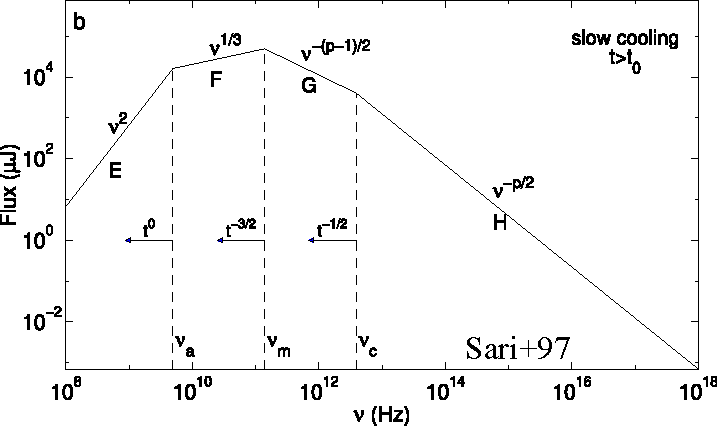
\includegraphics[height=5.0cm]{../figs/Sari97_spectrum_slow_cool.pdf}
                    %                        Overall, an afterglow spectrum has three characteristic frequencies: 
                    %                        (i) $\nu_i$ (injection break) at which most of the injected electrons radiate 
                    %                        (ii) $\nu_c$ (cooling break) at which for electrons expansion timescale is equal 
                    %                        to the radiative cooling timesacle
                    %                        (iii) $\nu_a$ an absorption break, below which synchrotron emission is absorbed by 
                    %                        electrons in free-free transitions in magnetic fields, (\ac{SSA}).
            }};
        }
    \end{tikzpicture}
\end{frame}